\documentclass[fleqn,final,5p,times]{elsarticle}

\usepackage[fleqn]{amsmath}
\usepackage{amssymb,amsthm,booktabs,array,tabularx,graphicx,xcolor}
\usepackage{siunitx}
\usepackage{microtype}
\usepackage{float}
\usepackage{pgfplots}
\usepgfplotslibrary{groupplots}
\pgfplotsset{compat=1.18}
\usepackage{hyperref}
\usepackage[switch]{lineno}
\setlength{\mathindent}{0pt}
\modulolinenumbers[5]
\setlength{\emergencystretch}{2em}
\setcounter{topnumber}{4}
\setcounter{bottomnumber}{2}
\setcounter{totalnumber}{6}
\setcounter{dbltopnumber}{3}
\renewcommand{\topfraction}{0.95}
\renewcommand{\bottomfraction}{0.85}
\renewcommand{\dbltopfraction}{0.92}
\renewcommand{\textfraction}{0.05}
\renewcommand{\floatpagefraction}{0.80}
\renewcommand{\dblfloatpagefraction}{0.75}
\setlength{\textfloatsep}{10pt plus 2pt minus 2pt}
\setlength{\dbltextfloatsep}{10pt plus 2pt minus 2pt}
\setlength{\floatsep}{6pt plus 1pt minus 1pt}
\setlength{\dblfloatsep}{6pt plus 1pt minus 1pt}
\hypersetup{hidelinks,hypertexnames=false}
\biboptions{numbers,sort&compress}

\newcommand{\R}{\mathbb{R}}
\newcommand{\W}{\mathcal{W}}
\newcommand{\abs}[1]{\left|#1\right|}
\newcommand{\RunningTitle}{Worst-case bounds for constrained AARB}
\newtheorem{proposition}{Proposition}
\newcommand{\inputsubmissiontable}[1]{%
  \IfFileExists{tables/#1}%
    {\input{tables/#1}}%
    {\input{#1}}}
\newcommand{\submissiongraphic}[2][]{%
  \IfFileExists{figures/#2}%
    {\includegraphics[#1]{figures/#2}}%
    {\includegraphics[#1]{#2}}}

\begin{document}
\begin{frontmatter}

\title{Worst-case transient bounds for constrained electrohydraulic active anti-roll-bar control of heavy vehicles}

\author[aff1]{Ali Salimnezhad}
\author[aff1]{Masoud Masih-Tehrani\corref{cor1}}
\ead{masih@iust.ac.ir}
\cortext[cor1]{Corresponding author.}
\affiliation[aff1]{organization={School of Automotive Engineering, Iran University of Science and Technology},
addressline={Tehran 16844},country={Iran}}

\begin{abstract}
Heavy-vehicle active anti-roll-bar controllers are usually assessed on prescribed manoeuvres, which do not establish worst-case load-transfer ratio (LTR) or actuator feasibility. This paper develops finite-horizon numerical upper bounds for a published ten-state electrohydraulic vehicle model. Sampled linear-quadratic-regulator (LQR) feedback is augmented by a causal finite-impulse-response (FIR) steering compensator. Exact first-order/zero-order-hold lifting and linear-programming support-function maximization evaluate the complete amplitude- and rate-bounded steering polytope; residual-corrected dual bounds and intersample remainders extend the results to continuous time. Reproduced active reference responses have RMS discrepancies below 5\%. At a \SI{20}{mA} current limit, the nominal balanced bound is 69.67\% below sampled LQR1. Rear-protected control reduces the nominal front bound by 66.77\%, and retains a 7.44\% reduction under LQR1's channel-wise current caps. Across 170 evaluated speed--payload plants, fixed balanced, rear-protected and scheduled designs reduce the maximum bound by 65.32\%, 62.70\% and 68.77\%, respectively, while satisfying the declared linear constraints. The retained zero-delay gain is unstable for every tested nonzero delay; a separately redesigned \SI{5}{ms} controller is stable at all 170 plants. Of 512 simultaneous $\pm5\%$ and 1024 $\pm10\%$ plant/controller stress records, 100 and 109, respectively, pass all sufficient verification gates. Most failures involve current authority, sampled stability or rear-margin loss. The numerical upper-bound results are pointwise for the declared linear plants and steering family.
\end{abstract}

\begin{keyword}
active anti-roll bar \sep heavy vehicle \sep electrohydraulic actuator \sep constrained control \sep worst-case analysis \sep numerical upper bounds
\end{keyword}

\end{frontmatter}
\linenumbers

\section{Introduction}
\label{sec:introduction}

Heavy vehicles are vulnerable to lateral load transfer because of their high centre of mass and narrow track. Active anti-roll bars (AARBs) oppose roll through front and rear actuators, but axle effects are coupled and actuator authority is finite: reducing body roll or front load transfer can worsen rear load transfer or demand infeasible current \cite{sampson2003achievable,sampson2003active}. This makes AARB design a constrained control problem in which peak performance, actuator feasibility and axle-wise behaviour must be considered together, rather than inferred from nominal tracking or stability alone.

Vehicle-control research has addressed this problem through LQR, differential-game and LMI designs \cite{yim2011game,yim2011lmi,yim2013}, hierarchical electrohydraulic and fault-tolerant control \cite{varga2015,nemeth2015,gaspar2005}, and LQR or $H_\infty$/LPV analysis of integrated lateral--roll--hydraulic models \cite{vu2017,vu2019lpv,vu2019leakage}. Other approaches include predictive rollover control \cite{jalali2018}, coordinated yaw--roll control \cite{liang2024}, sensing and observer design \cite{vu2023sensors,tan2024observer}, and predictive or adaptive chassis control \cite{oliveira2025,lu2025}. Recent work also studies roll-stiffness distribution and constrained learning \cite{sonnino2026,huang2026}; Ref.~\cite{tan2024book} and the commercial-vehicle survey in Ref.~\cite{chen2025survey} give broader accounts. Related IJRNC studies include LPV coordination of lateral and vertical vehicle dynamics \cite{fergani2017integrated}, sampled-data active-suspension control \cite{meng2018dualrate}, motion-mode decoupling for two-axle vehicles \cite{hu2020roll}, uncertainty- and delay-aware suspension control \cite{zhang2020semiactive}, and finite-frequency force tracking for electrohydraulic suspension \cite{zhang2024electrohydraulic}.

These methods address important controller-design, stability, performance and uncertainty questions, but they do not automatically provide the specific guarantee sought here: an upper bound on the largest finite-horizon load-transfer or actuator response over every steering history satisfying declared amplitude and rate limits. A finite set of prescribed manoeuvres supplies examples, not a bound over the admissible input set; likewise, sampled peak values alone can miss intersample extrema. Reference governors enforce constraints by reshaping commands \cite{berntorp2021,chakrabarty2023}, whereas the present problem leaves steering unchanged and asks whether the closed loop can tolerate the complete declared steering family.

For each evaluated speed--payload plant, the steering knots define a finite-dimensional polytope and the sampled controller combines state feedback with a causal finite-impulse-response (FIR) compensator. Exact mixed-hold lifting maps this polytope to the sampled states and outputs. Support-function linear programs then maximize output magnitudes: feasible primal witnesses give attainable lower bounds, while sign-constrained dual multipliers with an explicit stationarity-residual correction give numerical upper bounds on the sampled optima. An intersample remainder extends the upper bounds to continuous time. The worst-case optimization is performed offline; online execution retains only sampled matrix--vector and FIR operations, consistent with a compact constrained-control implementation \cite{lu2025}.

The robustness claim is deliberately scoped. It is with respect to the complete declared steering polytope and continuous finite-horizon time at each evaluated linear plant, not to a continuous uncertainty set of plant parameters. The 170-plant bank therefore gives pointwise numerical bounds, not an interval enclosure between plants; the analysis also does not establish nonlinear rollover prevention or experimental validation. This distinction makes the dual-bound calculation central: a numerical optimizer's candidate maximum alone is not an upper bound, whereas sign-constrained dual multipliers with the stationarity residual explicitly bounded, augmented by the intersample remainder, produce the reported numerical upper bound.

The main contributions are:
\begin{enumerate}
\item continuous-time worst-case load-transfer and actuator bounds over the complete amplitude- and rate-bounded steering polytope;
\item axle-specific and current-matched comparisons, including a one-sided rear non-degradation test;
\item synthesis and evaluation across 170 speed--payload plants, including 128 design-independent Sobol points; and
\item delay-aware redesign, nonlinear critical-case screening and a 1536-sample simultaneous plant--controller stress audit.
\end{enumerate}
Here, ``numerically certified'' is shorthand for a reproducible finite-precision bound calculation over the declared steering set and continuous finite-horizon time at each evaluated linear plant. The support, residual and intersample calculations use double-precision floating-point arithmetic without outward rounding or interval arithmetic. Thus the reported values are residual-corrected numerical upper bounds, not formally verified mathematical proofs or interval enclosures between plants; they do not establish nonlinear rollover prevention or experimental validation.

\section{Reproduced electrohydraulic benchmark}
\label{sec:model}

\subsection{Integrated model}

The state and input vectors follow \cite{vu2017}:
\begin{equation}
\begin{aligned}
x&=[\beta,r,\phi,p,\phi_{uF},\phi_{uR},P_F,X_{vF},P_R,X_{vR}]^\top,\\
u&=[u_F,u_R]^\top,
\end{aligned}
\label{eq:state}
\end{equation}
where $\beta$ is sideslip, $r$ yaw rate, $\phi$ sprung-body roll, $p=\dot\phi$, $\phi_{ui}$ unsprung roll, $P_i$ actuator pressure difference and $X_{vi}$ servo-valve displacement.
Table~\ref{tab:sign-convention} fixes the implemented coordinates. In the source-model balance equations, the front and rear unsprung gravity terms are respectively $+m_{uF}gh_u\phi_{uF}$ and $-m_{uR}gh_u\phi_{uR}$. When these equations are collected into the left-hand residual used by the implementation, their coefficients become $-m_{uF}gh_u\phi_{uF}$ and $+m_{uR}gh_u\phi_{uR}$. The rear residual sign therefore follows the published axle equation; it does not arise from a negative $g$. This axle-specific convention is retained in the archived model, and changing it would define a different plant.

\begin{table*}[t]
\centering\small
\caption{Implemented coordinates and sign conventions.}
\label{tab:sign-convention}
\begin{tabularx}{.92\textwidth}{@{}lX@{}}
\toprule
Quantity & Positive convention\\
\midrule
$x_v,y_v,z_v$ & Forward, left and upward, respectively\\
$\delta,\beta$ & Left steering and left lateral velocity\\
$r$ & Right-hand rotation about $+z_v$\\
$\phi,p,\phi_{uF},\phi_{uR}$ & Right-hand rotation about $+x_v$\\
$g$ & Positive magnitude; acceleration is $-g\mathbf e_{z_v}$\\
$P_i,u_i,T_i$ & Positive through the stated valve and torque equations\\
\bottomrule
\end{tabularx}
\end{table*}

At a fixed longitudinal speed, the vehicle and actuator equations form
\begin{equation}
\begin{alignedat}{1}
&E(\theta)\dot x=F(\theta)x+G(\theta)u+H_\delta(\theta)\delta,
\\[1em]
&\dot x=A(\theta)x+B(\theta)u+D(\theta)\delta,
\end{alignedat}
\label{eq:ss}
\end{equation}
where $\theta$ collects speed and vehicle parameters, $E,F,G,H_\delta$ are the assembled descriptor matrices, and $A=E^{-1}F$, $B=E^{-1}G$, $D=E^{-1}H_\delta$. The hydraulic dynamics at axle $i\in\{F,R\}$ are
{\small
\begin{equation}
\begin{alignedat}{1}
&\frac{V_t}{4\beta_e}\dot P_i+(K_P+C_{tp})P_i-K_xX_{vi}+A_p\ell_a(p-\dot\phi_{ui})=0,\\
&\dot X_{vi}=-X_{vi}/\tau_v+K_vu_i/\tau_v.
\end{alignedat}
\label{eq:hydraulic}
\end{equation}
}
The axle roll moment is $T_i=2\ell_aA_pP_i$, where $\ell_a$ is the effective moment arm of either actuator in the equal-and-opposite force pair (half the force-line separation in this representation). The normalized front and rear load-transfer ratios (LTRs) are
\begin{equation}
R_F=\frac{k_{tF}\phi_{uF}}{l_wmg\,l_R/(l_F+l_R)},\qquad
R_R=\frac{k_{tR}\phi_{uR}}{l_wmg\,l_F/(l_F+l_R)}.
\label{eq:ltr}
\end{equation}
where $m$ is total mass, $l_w$ is half track width, $l_F$ and $l_R$ locate the centre of mass relative to the axles, and $k_{tF},k_{tR}$ are tyre roll stiffnesses. The implementation assembles the published scalar residual equations and solves for their derivatives; no state-space matrix is fitted to response data. Complete equations and parameters, including the reconstruction assumption $\ell_a=\SI{0.50}{m}$ for the effective per-actuator moment arm, are given in the Supplementary Material; this value is not presented as a measured vehicle dimension.

LQR1 denotes the published continuous-time full-state LQR baseline \cite{vu2017}, using unit physical weights on body roll, both LTRs, both suspension relative-roll outputs and both actuator currents. Its gain is held between \SI{20}{ms} updates in the finite-horizon study. The exact cost and implementation details are reported in the Supplementary Material. This baseline is distinct from the 48-point sampled-data LQR tuning grid used later for an additional comparator.

\subsection{Reference-simulation reproduction}
\label{sec:validation}

Before controller synthesis, implementation fidelity was assessed independently against the published simulation. The protocol follows the reference study: \SI{70}{km/h}, zero initial state, a \SI{10}{s} horizon and a \SI{1}{ms} output interval. The steering input and comparison curves were digitized from Figs. 7 and 8 of \cite{vu2017}; no output amplitude scaling or time shift was applied.

Table~\ref{tab:validation} and Fig.~\ref{fig:validation} show active-response RMS discrepancies below 5\%; peak-normalized waveform errors for $R_F$, $R_R$, $u_F$ and $u_R$ are 0.19\%, 1.22\%, 1.63\% and 0.43\%. The 8.99\% passive rear discrepancy is not calibrated away. This is numerical reproduction, not experimental validation.

\begin{table}[t]
\centering
\caption{RMS comparison with selected published reference responses.}
\label{tab:validation}
\begin{tabular}{lrrr}
\toprule
Quantity & Reference & Present model & Error (\%)\\
\midrule
Passive $R_F$ & 0.2927 & 0.29649 & 1.30\\
Passive $R_R$ & 0.3413 & 0.37198 & 8.99\\
LQR1 $R_F$ & 0.0940 & 0.09099 & 3.20\\
LQR1 $R_R$ & 0.0126 & 0.01221 & 3.06\\
LQR1 $u_F$ (mA) & 0.33114 & 0.31478 & 4.94\\
LQR1 $u_R$ (mA) & 1.6000 & 1.58417 & 0.99\\
\bottomrule
\end{tabular}
\end{table}

\begin{figure*}[t]
\centering
\submissiongraphic[width=.76\textwidth]{reference_validation.png}
\caption{Reproduction of the published reference simulation: axle load transfers and actuator currents. Solid curves are recomputed responses and dashed curves are digitized reference traces. The active responses agree more closely than the passive responses.}
\label{fig:validation}
\end{figure*}

\section{Constrained transient-performance problem}
\label{sec:problem}

\subsection{Steering family and output limits}

The design horizon is $T_h=\SI{4}{s}$ and the controller update period is $h_s=\SI{20}{ms}$. Steering is piecewise linear between sampling knots,
\begin{equation}
\begin{aligned}
\delta_k&=\delta_{\max}w_k,\\
\W&=\{w:\ w_0=0,\ |w_k|\le1,\ |w_k-w_{k-1}|\le\eta\},
\end{aligned}
\label{eq:steering-set}
\end{equation}
with $\delta_{\max}=2^\circ$ and normalized rate increment $\eta=5^\circ\!/{\rm s}\times h_s/2^\circ=0.05$. Currents are zero-order held. The initial state is zero.

The primary outputs are $R_F$ and $R_R$. Actuator force $A_pP_i$, spool displacement $X_{vi}$, load flow $K_xX_{vi}-K_PP_i$ and suspension relative roll $\ell_a(\phi-\phi_{ui})$ are monitored together with body roll, tyre slip and sideslip. Table~\ref{tab:limits} gives the declared limits. The current rating is varied in the nominal authority study and is \SI{20}{mA} elsewhere.

\begin{table}[t]
\centering
\caption{Declared continuous-time constraints for the certification study.}
\label{tab:limits}
\begin{tabular}{lr}
\toprule
Output & Magnitude limit\\
\midrule
Current, each channel & \SI{20}{mA}\\
Actuator force, each channel & \SI{120}{kN}\\
Spool displacement & \SI{0.485}{mm}\\
Load flow & \SI{132}{L/min}\\
Suspension relative roll & $7^\circ$\\
Tyre slip & $3^\circ$\\
Body roll & $5^\circ$\\
Sideslip & $3^\circ$\\
\bottomrule
\end{tabular}
\end{table}

For controller coefficients $f$ and plant $\theta$, define the axle-wise peak bounds
\begin{equation}
U_i(f,\theta)=\sup_{w\in\W}\max_{t\in[0,T_h]}\abs{R_i(t;w,f,\theta)},
\qquad i\in\{F,R\}.
\label{eq:axle-objective}
\end{equation}
The balanced objective minimizes $\max(U_F,U_R)$. The rear-protected design instead minimizes $U_F$ subject to $U_R$ not exceeding the corresponding LQR1 value and all outputs satisfying Table~\ref{tab:limits}.

\subsection{Causal controller and exact lifting}

The control law combines a stabilizing sampled state feedback with causal steering-history compensation:
\begin{equation}
\begin{aligned}
u_k&=-Kx_k+i_0\sum_{j=1}^{6}f_jw_{k-d_j},\\
d_j&\in\{0,2,5,10,20,40\},\qquad i_0=\SI{20}{mA}.
\end{aligned}
\label{eq:policy}
\end{equation}
The two components of each $f_j$ command the front and rear channels. Only current and past steering knots are used. Exact matrix-exponential propagation with first-order-held steering and zero-order-held current gives
\begin{equation}
x_{k+1}=A_dx_k+B_du_k+G_0\delta_k+G_1\delta_{k+1}.
\label{eq:lift}
\end{equation}
Although $\delta_{k+1}$ appears in the plant propagation, $u_k$ is selected before it is available; the implemented controller has no preview.

The twelve FIR coefficients are restricted to the declared box $[-50,50]^{12}$. This finite-dimensional family is used for synthesis and for the family-specific lower bound; it is not treated as the set of all causal controllers.

At any output phase $q$ inside a control interval, the lifted response is affine in the steering knots and controller coefficients. For fixed $f$ it can be written as $y_{qk}=g_{qk}(f)^\top w$. The worst positive value is the linear program
\begin{equation}
\sigma_\W(g)=\max_w\{g^\top w:A_ww\le b_w,\ -\mathbf{1}\le w\le\mathbf{1}\}.
\label{eq:support}
\end{equation}
The rows of $A_w w\le b_w$ impose the fixed initial knot and rate constraints; the explicit box bounds impose the knot-amplitude limits. The support solve is passed to the LP solver as $\min_w -g^\top w$ subject to these constraints. Let $y^{\rm raw}$ denote the inequality marginals returned for this minimization. Under the SciPy/HiGHS minimization convention these multipliers must satisfy $y\le0$; the implementation enforces this sign by setting $y=\min(y^{\rm raw},0)$ componentwise, and defines the stationarity residual
\begin{equation}
r_d=-g-A_w^\top y.
\end{equation}
For any feasible $w$, $y^\top(A_w w-b_w)\ge0$ and $|r_d^\top w|\le\|r_d\|_1$, so
\begin{equation}
\begin{aligned}
-g^\top w&=r_d^\top w+y^\top A_w w\\
&\ge -\|r_d\|_1+b_w^\top y,\\
\sigma_\W(g)&\le-b_w^\top y+\|r_d\|_1.
\end{aligned}
\label{eq:support-dual-correction}
\end{equation}
Negative peaks use $-g$. The bound includes the complete computed stationarity residual rather than treating a small solver residual as zero. A support solve is retained only after a successful solver status. The archived computation uses SciPy 1.17.0 ``linprog'' with HiGHS: primal and dual feasibility tolerances are the interface defaults of $10^{-7}$ and the interior-point optimality tolerance is $10^{-8}$; no custom tolerance overrides are passed. The support routine tries ``highs'', then ``highs-ds'' with presolve disabled, and then ``highs-ipm'' with presolve enabled. These are solver stopping tolerances, not allowances used in the residual correction. In the independent one-sided rear audit, a primal steering witness is separately accepted only when its maximum rate-constraint and box violations are each no greater than $5\times10^{-8}$; this witness-feasibility threshold is distinct from the HiGHS tolerances.

The master design LP contains only a subset of worst-case steering witnesses; a separation loop alternates between solving the master and adding the most violated witness. For a master minimization $\min_{\ell\le\xi\le u}c^\top\xi$ subject to $A\xi\le b$, let $y\le0$ be its inequality marginals and define $r_m=c-A^\top y$. The residual-corrected lower bound used for the master objective is
\begin{equation}
L_m=b^\top y+\sum_j\min\{r_{m,j}\ell_j,r_{m,j}u_j\}.
\label{eq:master-dual-correction}
\end{equation}
The same sign convention and full-residual correction apply; the master bound is a lower bound for the finite master problem, and the exchange procedure supplies the stated FIR-family comparison. This is a standard affine-policy robust optimization construction \cite{goulart2006,boyd2004}, but here it retains the complete integrated hydraulic model and distinct steering/current holds.

Two different lower-bound questions are retained. Removing the design margin and using the residual-corrected master dual gives a lower bound $L_{\mathcal F}$ on the optimum within the declared FIR family. A broader nonanticipative scenario-tree relaxation gives $L_G$ for all causal sampled policies represented by the tree. The tree omits most steering histories and the non-current constraints, so $L_G$ is a valid but intentionally loose diagnostic; it must not be interpreted as a solved global optimum.

\subsection{Continuous-time and one-sided numerical bounds}

The corrected support expression in Eq.~\eqref{eq:support-dual-correction} bounds each sampled support value in exact arithmetic; its reported evaluation is finite-precision numerical evidence, not an outward-rounded proof. Let $\bar U_{i,\Delta_q}$ denote the largest corrected support value on a phase grid with spacing $\Delta_q$. Within each current-hold interval, the FOH steering and ZOH current admit an augmented linear flow $\dot z=Jz$ and output $y=C_a z$. The resulting output is twice differentiable on each interval. A componentwise matrix-exponential envelope gives a bound $M_y(f,\theta)$ on $|\ddot y|$; linear interpolation between adjacent phase samples then gives the quadratic remainder $\epsilon_i(\Delta_q,f,\theta)=M_{y,i}(f,\theta)\Delta_q^2/8$, with $M_y(f,\theta)=|C_aJ^2|\exp(|J|h_s)\bar v$ (details are in the Supplementary Material). Thus,
\begin{equation}
U_i(f,\theta)\le \bar U_{i,\Delta_q}(f,\theta)+\epsilon_i(\Delta_q,f,\theta).
\label{eq:continuous-bound}
\end{equation}
Mesh refinement is applied to the final controller rather than changing the update period.

Rear non-degradation requires a one-sided comparison. For each plant, the proposed continuous upper bound is compared with the largest objective attained by a feasible LQR1 steering witness on the fine grid:
\begin{equation}
\overline U_R^{P}=\bar U_{R,\Delta_q}^{P}+\epsilon_R^{P},\qquad
\underline U_R^{L}=\max_{q,k}\sigma_{\W}^{\rm feas}(g_{qk}^{L}).
\label{eq:rear-proof}
\end{equation}
If $\overline U_R^{P}\le\underline U_R^{L}$, the proposed continuous-time rear peak cannot exceed the LQR1 peak. This avoids drawing a dominance conclusion from two independently conservative upper bounds.

\section{Implementation architecture and numerical-bound scope}
\label{sec:architecture-scope}

{Figure~\ref{fig:certification-architecture} separates offline numerical-bound evaluation from the online policy. Offline steps construct the lifted maps, solve support and exchange LPs, and audit versioned artifacts. Online, state and steering history feed the optional schedule, feedback and causal FIR blocks before the zero-order-held actuators. The nonlinear surrogate remains outside the evaluated linear model.}

\begin{figure*}[!t]
\centering
% Use the opaque raster export here because some embedded PDF viewers render
% the transparency layers of the vector original as a blank page.
\submissiongraphic[width=.96\textwidth]{certification_architecture.png}
\caption{Reproducible architecture of the certification study. The upper lane is executed offline; the lower lane is the sampled controller. The current block is a verified guard in the linear study, whereas explicit saturation is used only in the nonlinear screening surrogate.}
\label{fig:certification-architecture}
\end{figure*}

{Table~\ref{tab:certificate-scope} states the claim boundary: ``numerically certified'' means a residual-corrected finite-precision bound for the declared steering family and continuous finite horizon at each evaluated linear plant. No outward-rounded arithmetic is used, so this is not a formally verified proof, interval parameter enclosure, nonlinear rollover guarantee or experimental result.}

\begin{table*}[!t]
\centering\scriptsize
\caption{Scope of the numerical certificate and explicit non-claims.}
\label{tab:certificate-scope}
\begin{tabularx}{\textwidth}{@{}>{\raggedright\arraybackslash}p{.15\textwidth}>{\raggedright\arraybackslash}X>{\raggedright\arraybackslash}X@{}}
\toprule
Dimension & Included in the evidence & Excluded from the claim\\
\midrule
\inputsubmissiontable{certificate_scope.tex}
\end{tabularx}
\end{table*}

\section{Operating-envelope construction}
\label{sec:envelope}

The nominal model uses \SI{70}{km/h}. To evaluate generalization, speed varies over $v\in[50,75]$ km/h. Added payload mass is $m_p=\mu m_{s0}$ with $\mu\in[0,0.10]$, and payload height is $h_p\in[h_0,\SI{1.80}{m}]$. The idealized payload is placed on the vehicle centreline at the nominal longitudinal centre of mass, and its intrinsic inertia tensor per unit mass is set equal to that of the nominal sprung body. Thus its intrinsic contributions are $\mu I_{xx0}$, $\mu I_{xz0}$ and $\mu I_{zz0}$. The only centroid offset is vertical, so the parallel-axis correction contributes to $I_{xx}$ but not to $I_{xz}$ or $I_{zz}$. The resulting coupled parameters are
\begin{equation}
\begin{alignedat}{1}
&m_s=m_{s0}+m_p,\\
&h=\frac{m_{s0}h_0+m_ph_p}{m_s},\\
&I_{xx}=(1+\mu)I_{xx0}+m_{s0}(h_0-h)^2+m_p(h_p-h)^2,\\
&I_{xz}=(1+\mu)I_{xz0},\qquad I_{zz}=(1+\mu)I_{zz0}.
\end{alignedat}
\label{eq:payload}
\end{equation}
At $h_p=h_0$, all three sprung-body inertias scale by $1+\mu$. The family is mechanically coupled but is an idealized assumption, not a payload-specific measured inertia model or a family identified from a particular fleet.

The upper speed is a declared linear-model boundary, not a physical maximum-speed claim. In the precursor screen, fixed LQR1 remains within the selected model-domain limits at \SI{75}{km/h}, whereas loaded cases at 80 and \SI{90}{km/h} exceed the $3^\circ$ front-tyre-slip guard by approximately 2\% and 25\%, respectively; details are retained in the Supplementary Material.

The fixed rear-protected controller is synthesized jointly on nine skeleton models: speeds 50, 62.5 and \SI{75}{km/h}, each at nominal load, $(\mu,h_p)=(0.10,h_0)$ and $(0.10,\SI{1.80}{m})$. The fixed controllers retain the nominal 70 km/h gain. The scheduled controller linearly interpolates both $K$ and the FIR coefficients between independently synthesized nodes at 50, 70 and \SI{75}{km/h}.

Verification uses two parameter collections. A 42-point structured grid contains six speeds, nominal load, and all combinations of $\mu\in\{0.05,0.10\}$ with $h_p\in\{1.15,1.475,1.80\}$ m. A separate 128-point scrambled-Sobol set \cite{sobol1967,owen1998} is generated with a fixed seed and is never used for synthesis. For every plant, the steering support LP covers the complete set \eqref{eq:steering-set}; the Sobol sampling applies to vehicle parameters, not steering histories. Broad screening uses 21 phases per interval and the rear dominance audit uses 81 phases.

\section{Results}
\label{sec:results}

Results progress from nominal comparison to envelope, dominance, numerical, sensitivity, latency and implementation audits. Unless stated otherwise, each peak is a continuous-time upper bound over Eq.~\eqref{eq:steering-set}, not a single-manoeuvre maximum.

\subsection{Nominal performance and comparison fairness}

At 70 km/h and 20 mA, the balanced worst-axle bound is 0.046115 versus 0.152022 for sampled LQR1 on the 41-phase nominal grid, a 69.67\% reduction. The FIR-family lower bound is 0.045757, giving a 0.776\% bracket. Table~\ref{tab:authority-brackets} shows similarly narrow family brackets at all ratings, whereas the smaller scenario-tree bounds leave all-policy optimality unresolved.

\begin{table*}[!t]
\centering
\caption{Nominal performance bounds and comparison with a discrete-LQR tuning grid. $L_G$ is the scenario-tree lower bound for the broader causal-policy relaxation; $L_{\mathcal F}$ applies only to the declared FIR family.}
\label{tab:authority-brackets}
\begin{tabular}{rrrrrr}
\toprule
Current limit (mA) & $L_G$ & $L_{\mathcal F}$ & Proposed $U$ & Family width (\%) & Best discrete LQR $U$\\
\midrule
5  & 0.010595 & 0.139995 & 0.140227 & 0.166 & 0.185032\\
10 & 0.006656 & 0.102074 & 0.102256 & 0.178 & 0.158239\\
20 & 0.003456 & 0.045757 & 0.046115 & 0.776 & 0.158239\\
\bottomrule
\end{tabular}
\end{table*}

LQR1 is infeasible at 5 mA and is not clipped. The 81-phase axle-wise comparison in Table~\ref{tab:nominal-fairness} reports 0.151990 for LQR1, refining the 41-phase nominal-grid value of 0.152022 above. ``Best discrete LQR'' is the best feasible member of a separate 48-point sampled-data tuning grid; it is an additional comparator, not a bound over all LQR tunings.

Table~\ref{tab:nominal-fairness} and Fig.~\ref{fig:nominal-fairness} separate the axles. At 20 mA, rear-protected control reduces the front bound by 66.77\% and slightly decreases the rear bound. Under LQR1's exact marginal caps, 5.2736 and 4.1511 mA, the front reduction remains 7.44\% without rear degradation. The full-authority result therefore combines controller structure with additional current use.

\begin{table*}[!t]
\centering
\caption{Nominal axle-wise worst-case bounds and marginal current demand at \SI{20}{mA} (81 phases). Current caps are marginal values; front and rear maxima need not share one steering history.}
\label{tab:nominal-fairness}
\begin{tabular}{lrrrrrr}
\toprule
Controller & $U_F$ & $U_R$ & $I_F$ (mA) & $I_R$ (mA) & $\max(U_F,U_R)$ & Front reduction (\%)\\
\midrule
Sampled LQR1 & 0.151990 & 0.020535 & 5.2736 & 4.1511 & 0.151990 & 0.00\\
Equal-current balanced & 0.138701 & 0.028989 & 5.2736 & 4.1511 & 0.138701 & 8.74\\
Equal-current rear-protected & 0.140683 & 0.020530 & 5.2736 & 4.1511 & 0.140683 & 7.44\\
20 mA rear-protected & 0.050503 & 0.020438 & 19.9600 & 19.9601 & 0.050503 & 66.77\\
\bottomrule
\end{tabular}
\end{table*}

\begin{figure*}[!t]
\centering
\submissiongraphic[width=.88\textwidth]{nominal_fairness.png}
\caption{Nominal axle-wise bounds under matched and full current authority. Matching the LQR1 peak-current caps gives a smaller but nonzero dominance result; the \SI{20}{mA} design uses nearly the full declared authority.}
\label{fig:nominal-fairness}
\end{figure*}

All actuator constraints remain feasible (Table~\ref{tab:actuator-audit}); marginal maxima need not share one steering history. Body roll and sideslip are bounded by $0.3758^\circ$ and $1.2799^\circ$.

\begin{table}[!t]
\centering\small
\caption{Nominal continuous-time output audit for the 20 mA rear-protected controller.}
\label{tab:actuator-audit}
\begin{tabular}{lrrr}
\toprule
Quantity & Front & Rear & Limit\\
\midrule
Current (mA) & 19.9600 & 19.9601 & 20\\
Force (kN) & 21.395 & 26.774 & 120\\
Spool (mm) & 0.3948 & 0.3943 & 0.485\\
Load flow (L/min) & 56.157 & 56.482 & 132\\
Suspension roll (deg) & 0.3588 & 0.3336 & 7\\
Tyre slip (deg) & 2.2255 & 2.0583 & 3\\
\bottomrule
\end{tabular}
\end{table}

Mesh refinement leaves the 20 ms controller unchanged (Table~\ref{tab:mesh-refinement}). The conservative five-phase failure is caused by its coarse intersample remainder, not an observed saturation.

\begin{table}[!t]
\centering\scriptsize
\caption{Certification-mesh refinement for the same nominal 20 mA controller.}
\label{tab:mesh-refinement}
\begin{tabular}{rrrrr}
\toprule
Phases & Spacing (ms) & Grid peak & Continuous $U$ & Max. utilization\\
\midrule
5  & 5.00 & 0.0459432 & 0.0630916 & 1.224119\\
9  & 2.50 & 0.0459434 & 0.0502304 & 0.998001\\
21 & 1.00 & 0.0459432 & 0.0466292 & 0.998001\\
41 & 0.50 & 0.0459434 & 0.0461149 & 0.998001\\
81 & 0.25 & 0.0459439 & 0.0459868 & 0.998001\\
\bottomrule
\end{tabular}
\end{table}

\subsection{Operating-envelope performance}

Over 42 structured and 128 design-independent plants, rear protection raises the fixed-controller maximum from 0.054784 to 0.058921, whereas scheduling lowers it to 0.049333, 9.95\% below fixed balanced control (Table~\ref{tab:envelope-summary} and Fig.~\ref{fig:envelope-summary}). All evaluated loops are stable and satisfy the non-LTR constraints.

\begin{table*}[!t]
\centering
\caption{Operating-envelope performance over 170 evaluated linear plants. Reductions compare continuous-time upper bounds with fixed LQR1.}
\label{tab:envelope-summary}
\begin{tabular}{lrrrrl}
\toprule
Controller & Worst bound & Reduction (\%) & Max. utilization & Max. spectral radius & Rear protected\\
\midrule
Fixed LQR1 & 0.157957 & 0.00 & 0.909548 & 0.901008 & Reference\\
Fixed balanced & 0.054784 & 65.32 & 0.994002 & 0.901008 & No\\
Fixed rear-protected & 0.058921 & 62.70 & 0.985006 & 0.901008 & Yes\\
Speed scheduled & 0.049333 & 68.77 & 0.997310 & 0.901346 & No\\
\bottomrule
\end{tabular}
\end{table*}

\begin{figure*}[!t]
\centering
\submissiongraphic[width=.96\textwidth]{operating_envelope_summary.png}
\caption{Operating-envelope results for 170 evaluated linear plants: 42 structured points from six speeds (50--75~km/h), nominal load, and all combinations of added-mass fraction $\mu\in\{0.05,0.10\}$ and payload height $h_p\in\{1.15,1.475,1.80\}$~m, plus 128 design-independent Sobol points. (a) Maximum worst-axle upper bound over structured payloads at each speed; (b) empirical CDF of worst-axle upper bounds over the Sobol points. In (a)--(b), gray, blue, orange and green denote fixed LQR1, fixed balanced, fixed rear-protected and speed-scheduled control, respectively. (c) One-sided rear margin over the 170-plant bank; positive values mean the proposed upper bound is below the feasible LQR1 lower witness. Point color indicates added-mass fraction. (d) Largest normalized non-LTR utilization over structured payloads for fixed balanced (blue), fixed rear-protected (orange) and scheduled (green) control; the dashed line marks the unit limit. Every bound uses worst-case steering.}
\label{fig:envelope-summary}
\end{figure*}

For LQR1, fixed balanced, fixed rear-protected and scheduled control, the structured maxima are 0.157957, 0.054784, 0.058921 and 0.049333; Sobol maxima are 0.156823, 0.054330, 0.058371 and 0.048975. The lower holdout values are not an interval proof.

Sobol-point Spearman coefficients, ordered as $(v,\mu,h_p)$, are $(0.895,-0.432,0.011)$ for LQR1 and $(-0.019,-0.316,0.019)$ for fixed balanced control. Rear-protected and scheduled values are $(0.987,-0.149,0.010)$ and $(0.957,-0.265,0.031)$. These are rank descriptors, not causal decompositions.

\subsection{Rear-axle dominance and scheduling trade-off}

Because independent upper bounds have different intersample corrections, the bank-wide comparison uses Eq.~\eqref{eq:rear-proof} with 81 phases (Fig.~\ref{fig:rear-certificate}). All 170 plants pass. At the limiting point $(75\ \mathrm{km/h},0.05,1.475\ \mathrm{m})$, the proposed upper bound is 0.01726882 and the feasible LQR1 lower witness is 0.01732703, giving $5.82\times10^{-5}$ absolute or 0.336\% relative margin. Independent reconstruction agrees to machine precision.

\begin{figure*}[!t]
\centering
\submissiongraphic[width=.86\textwidth]{rear_certificate.png}
\caption{One-sided rear-axle audit. Every proposed continuous upper bound is below the corresponding feasible sampled LQR1 lower bound. The right panel shows the distribution of relative margins.}
\label{fig:rear-certificate}
\end{figure*}

Scheduling improves fixed balanced control by 10.34\% on average and 29.83\% at 50 km/h nominal load, but one Sobol point changes by $-0.18$\%; it therefore improves the envelope maximum without pointwise dominance. Rear protection instead trades a higher aggregate bound for axle-wise dominance.

\subsection{Numerical audit and rear-bound error budget}

The HiGHS exchange design \cite{highs2018,scipy2020} converges in 28 iterations. Its maximum dual-residual correction is below $2.1\times10^{-7}$; exact-hold and implicit-integration checks agree within $5\times10^{-13}$ in scaled states. {Six error-budget, four reserve-design, four envelope and ten legacy tests pass.}

{Table~\ref{tab:rear-error-budget} and Fig.~\ref{fig:rear-error-budget} decompose the limiting numerical bound comparison into primal sampled gap, residual-dual budget and intersample remainder. The 41-phase result is inconclusive; the residual-corrected comparison is positive at 81 phases, while 161- and 321-phase refinements raise the margin to 0.523\% and 0.570\%.}

\begin{table*}[!t]
\centering\small
\caption{Error budget for the limiting one-sided rear-axle certificate. A negative 41-phase margin denotes an inconclusive coarse bound, not a violating trajectory.}
\label{tab:rear-error-budget}
\inputsubmissiontable{rear_error_budget_table.tex}
\end{table*}

\begin{figure*}[!t]
\centering
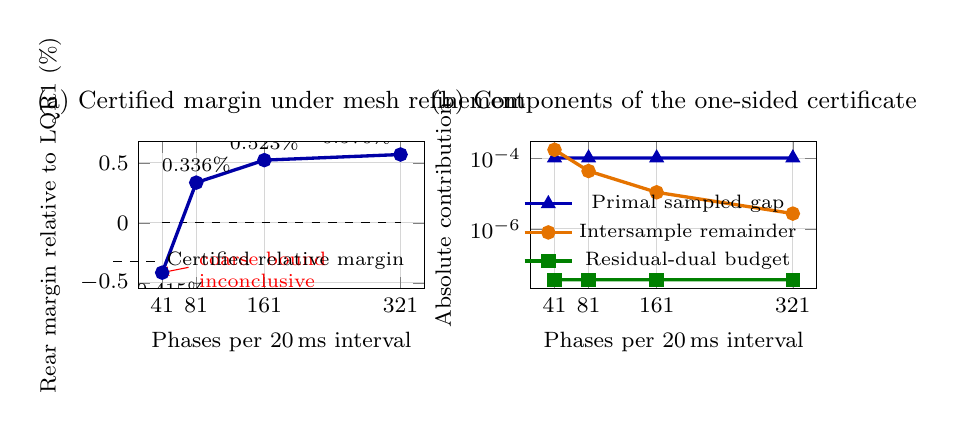
\begin{tikzpicture}
\begin{groupplot}[
  group style={group size=2 by 1,horizontal sep=1.35cm},
  width=.43\textwidth,
  height=.285\textwidth,
  xlabel={Phases per \SI{20}{ms} interval},
  xtick={41,81,161,321},
  tick label style={font=\footnotesize},
  label style={font=\footnotesize},
  title style={font=\small},
  legend style={font=\scriptsize,draw=none,fill=none},
  grid=both,
  major grid style={black!16},
  minor grid style={black!7},
]
\nextgroupplot[
  title={(a) Certified margin under mesh refinement},
  ylabel={Rear margin relative to LQR1 (\%)},
  ymin=-0.55,ymax=0.68,
  legend style={at={(0.98,0.05)},anchor=south east},
]
\addplot[black,dashed,thin,domain=41:321,samples=2] {0};
\addplot[blue!65!black,very thick,mark=*] coordinates {
  (41,-0.414537) (81,0.335966) (161,0.523342) (321,0.570269)
};
\addlegendentry{Certified relative margin}
\node[font=\scriptsize,anchor=north] at (axis cs:41,-0.414537) {$-0.415\%$};
\node[font=\scriptsize,anchor=south] at (axis cs:81,0.335966) {$0.336\%$};
\node[font=\scriptsize,anchor=south] at (axis cs:161,0.523342) {$0.523\%$};
\node[font=\scriptsize,anchor=south east] at (axis cs:321,0.570269) {$0.570\%$};
\node[red,font=\scriptsize,align=left,anchor=west]
  at (axis cs:73,-0.39) {coarse bound\\inconclusive};
\draw[red,->,thin] (axis cs:72,-0.37) -- (axis cs:43,-0.411);

\nextgroupplot[
  title={(b) Components of the one-sided certificate},
  ylabel={Absolute contribution},
  ymode=log,
  ymin=2e-8,ymax=3e-4,
  legend style={at={(0.98,0.05)},anchor=south east},
]
\addplot[blue!70!black,very thick,mark=triangle*] coordinates {
  (41,1.016316e-4) (81,1.016048e-4)
  (161,1.015548e-4) (321,1.015567e-4)
};
\addlegendentry{Primal sampled gap}
\addplot[orange!90!black,very thick,mark=*] coordinates {
  (41,1.734224e-4) (81,4.335560e-5)
  (161,1.083890e-5) (321,2.709725e-6)
};
\addlegendentry{Intersample remainder}
\addplot[green!50!black,very thick,mark=square*] coordinates {
  (41,3.624268e-8) (81,3.630557e-8)
  (161,3.627410e-8) (321,3.627410e-8)
};
\addlegendentry{Residual-dual budget}
\end{groupplot}
\end{tikzpicture}
\caption{Mesh refinement of the limiting one-sided rear certificate. Panel (a) distinguishes the inconclusive 41-phase bound from the positive 81-phase and finer certificates. Panel (b) shows the nearly mesh-independent sampled gap and residual-dual budget together with the quadratically decreasing intersample remainder.}
\label{fig:rear-error-budget}
\end{figure*}

{At 321 phases, the sampled gap, dual budget and remainder are $1.01557\times10^{-4}$, $3.6274\times10^{-8}$ and $2.71\times10^{-6}$, leaving $9.88\times10^{-5}$. Automatic, dual-simplex and interior-point HiGHS solutions are feasible and vary by at most $2.41\times10^{-8}$, over 4100 times less than this margin. The budget covers numerical resolution, not plant uncertainty.}

\subsection{Rear-reserve redesign and controller selection}

{To enlarge the small original rear margin, fixed compensators requesting 1\%, 2\% and 5\% reserves were screened on 170 plants and audited at 81 phases (Table~\ref{tab:rear-reserve-tradeoff} and Fig.~\ref{fig:rear-reserve-tradeoff}); regenerated records and artifacts pass consistency checks.}

\begin{table*}[!t]
\centering\small
\caption{Rear-reserve trade-off over the 170 evaluated plants. Front cost is relative to the current rear-protected controller; utilization is normalized by the declared non-LTR limits.}
\label{tab:rear-reserve-tradeoff}
\begin{tabular}{lrrrrrr}
\toprule
Controller & Requested (\%) & Achieved (\%) & Worst front & Cost (\%) & Max. utilization & Max. $\rho$\\
\midrule
\inputsubmissiontable{table_rear_reserve_tradeoff.tex}
\end{tabular}
\end{table*}

\begin{figure*}[!t]
\centering
\submissiongraphic[width=.88\textwidth]{rear_reserve_tradeoff.png}
\caption{Trade-off obtained by deliberate rear-reserve redesign. Panel (a) shows the small front-performance price of increasing the certified minimum rear margin. Panel (b) gives the complete margin distributions over the same 170 evaluated plants.}
\label{fig:rear-reserve-tradeoff}
\end{figure*}

{All redesigns are feasible with maximum spectral radius 0.901008 and achieve 1.156\%, 2.126\% and 5.148\% minimum margins. The selected 5\% design raises the worst front bound from 0.058921 to 0.059092 (0.291\%) and reaches 0.985006 utilization. This remains a pointwise bank result.}

\subsection{Fixed-controller sensitivity}

{The selected 5\% controller is held fixed while FIR order, horizon, steering limits, delay and hydraulics vary (Tables~\ref{tab:sensitivity-fir-horizon}, \ref{tab:sensitivity-delay} and \ref{tab:sensitivity-hydraulic}; Figs.~\ref{fig:fixed-sensitivity} and \ref{fig:delay-hydraulic-sensitivity}). FIR, horizon and steering tests use 42 structured plants, hydraulics use nine skeleton plants and delay uses all 170; screening does not replace the 81-phase certificate.}

\begin{table*}[!t]
\centering\small
\caption{Sensitivity to FIR order, horizon and steering-family limits for the selected fixed 5\% reserve controller. All cases use 42 structured plants and 41 intersample phases and are stable ($\rho_{\max}=0.901008$). Values are tap counts, horizon in seconds, or steering amplitude/rate pairs in degrees and degrees per second. Rear margin is the minimum one-sided percentage; Pass requires output-limit satisfaction and rear non-degradation.}
\label{tab:sensitivity-fir-horizon}
\begin{tabular}{llrrrr}
\toprule
Study & Value & Worst front LTR & Rear margin (\%) & Max. utilization & Status\\
\midrule
\inputsubmissiontable{sensitivity_fir_horizon.tex}
\end{tabular}
\par\smallskip
{\footnotesize Status: Constraint = output-limit failure; Rear = rear non-degradation failure; Both = both. The six-tap row's 4.415\% margin is the 41-phase, 42-plant screen; Table~\ref{tab:rear-reserve-tradeoff} reports 5.148\% using 81 phases over 170 plants. These figures use different phase meshes and plant banks.}
\end{table*}

\begin{figure*}[!t]
\centering
\submissiongraphic[width=.92\textwidth]{fixed_sensitivity_summary.png}
\caption{Sensitivity of the selected fixed 5\% rear-reserve controller on 42 structured plants (six speeds, 50--75~km/h; nominal load plus $\mu\in\{0.05,0.10\}$ at $h_p\in\{1.15,1.475,1.80\}$~m), using 41 intersample phases. Unless varied, the horizon is \SI{4}{s} and steering limits are $2^\circ$ and $5^\circ/\mathrm{s}$. (a) FIR truncation: blue solid circles (left axis) give worst front LTR; orange dashed squares (right axis) give maximum normalized non-LTR utilization; the dotted line is the unit limit. (b) Worst front-LTR bound at horizons of 2, 4 and \SI{6}{s} (expanded scale; total spread $2.7\times10^{-7}$). (c,d) Nine steering families, with amplitude rows of 1, 2 and $3^\circ$ and rate columns of 2.5, 5 and $7.5^\circ/\mathrm{s}$: cells show maximum normalized utilization in (c) and minimum one-sided rear margin (\%) in (d). Positive rear margin means no degradation relative to LQR1; color bars show metric scales.}
\label{fig:fixed-sensitivity}
\end{figure*}

{Four taps are the smallest passing subset: its worst front bound and rear margin are 0.059554 and 4.432\%. Three taps reach 1.0067 utilization; one and two taps fail more strongly. Horizons from 2 to 6 s change the front bound by only $2.70\times10^{-7}$. Of nine steering families, only $(1^\circ,2.5^\circ/\mathrm{s})$, $(2^\circ,2.5^\circ/\mathrm{s})$ and $(2^\circ,5^\circ/\mathrm{s})$ pass; larger sets activate constraints, while $(1^\circ,5^\circ/\mathrm{s})$ degrades the rear axle.}

\begin{table}[!t]
\centering\small
\caption{Fixed-controller delay stability on 170 plants.}
\label{tab:sensitivity-delay}
\begin{tabular}{rrrrl}
\toprule
Delay (ms) & Min. $\rho$ & Max. $\rho$ & Stable & Status\\
\midrule
\inputsubmissiontable{sensitivity_delay.tex}
\end{tabular}
\end{table}

\begin{table*}[!t]
\centering\small
\caption{Fixed-controller sensitivity to hydraulic parameters on nine design-skeleton plants. ``Unstable cases'' lists factors producing $\rho\ge1$; other columns refer to stable cases.}
\label{tab:sensitivity-hydraulic}
\begin{tabular}{lrrrr}
\toprule
Parameter & Unstable cases & Worst stable utilization & Min. rear margin (\%) & Max. $\rho$\\
\midrule
\inputsubmissiontable{sensitivity_hydraulic.tex}
\end{tabular}
\end{table*}

\begin{figure*}[!t]
\centering
\submissiongraphic[width=.96\textwidth]{delay_hydraulic_summary.png}
\caption{Fixed-controller delay and hydraulic sensitivity. (a) Minimum (orange dashed squares) and maximum (blue solid circles) sampled closed-loop spectral radius over the 170 evaluated plants at common measurement delays of 0, 5, 10 and \SI{20}{ms}; the dotted line at $\rho=1$ is the Schur-stability boundary. (b) Maximum spectral radius over nine design-skeleton plants: speeds 50, 62.5 and 75~km/h at nominal load, $(\mu,h_p)=(0.10,h_0)$ and $(0.10,\SI{1.80}{m})$. Each marker corresponds to the indicated hydraulic-parameter factor relative to nominal. Blue circles pass stability, output-limit and rear-comparison checks; amber triangles are stable but fail an output or rear check; orange crosses are unstable ($\rho\ge1$). The dotted line again marks $\rho=1$. These hydraulic perturbations are diagnostic screens, not uncertainty guarantees.}
\label{fig:delay-hydraulic-sensitivity}
\end{figure*}

{The zero-delay maximum radius is 0.901. Delays of 5, 10 and 20 ms destabilize every plant, with maxima 1.216, 1.521 and 1.843. Seven hydraulic cases are unstable: $K_v$ factors 1.1 and 1.2, $\tau_v$ factors 0.8 and 0.9, $K_x=1.2$, $\beta_e=1.2$ and $V_t=0.8$. Some stable cases, especially piston-area variations, violate constraints or rear dominance; all tested $K_P$ and positive-leakage cases remain feasible. These are diagnostic, not uncertainty certificates.}

\subsection{Combined parameter--controller stress audit}

The selected 5\% rear-reserve controller is held fixed while operating conditions, 15 plant parameters, all 20 feedback-gain entries and all 12 FIR coefficients vary simultaneously. The operating coordinates $(v,\mu,h_p)$ span Section~\ref{sec:envelope}; derived mass and inertia terms are recomputed from Eq.~\eqref{eq:payload}. For Sobol coordinate $s_j\in[0,1)$ and stress amplitude $\varepsilon\in\{0.05,0.10\}$,
\begin{equation}
z_j=z_j^-+s_j(z_j^+-z_j^-),\qquad
q_j^{(\varepsilon)}=q_j^0\,[1+\varepsilon(2s_j-1)],
\label{eq:combined-uncertainty}
\end{equation}
where $z_j\in\{v,\mu,h_p\}$ and $q_j$ is a plant or controller coefficient. Each record is therefore a 50-dimensional coordinate-wise box perturbation without assumed correlations or probabilities. Independent Owen-scrambled Sobol nets \cite{sobol1967,owen1998} use $512=2^9$ samples at $\pm5\%$ and $1024=2^{10}$ at $\pm10\%$, with fixed seeds 2026092705 and 2026092710. These are engineering stress brackets, not estimated tolerances or confidence intervals.

A record passes the sufficient verification gates only if the solver completes, the proposed and nominal-coefficient LQR1 loops are stable on the same perturbed plant, every normalized non-LTR bound is at most one, and the one-sided rear reserve $m_R=(\underline U_R^{L}-\overline U_R^{P})/\underline U_R^{L}$ is positive. Stable cases use 21-phase output and 41-phase rear screens; limiting records are recomputed with 41/81 phases. No tolerance-relaxed classification is used. Table~\ref{tab:combined-robustness} and Fig.~\ref{fig:combined-robustness} summarize the overlapping gates; protocol details and the recorded numerical environment are supplied in the Supplementary Material.

\begin{table*}[!t]
\centering\scriptsize
\caption{Combined operating-condition, plant and controller stress audit. Stable, feasible and rear-certificate counts overlap; ``Pass'' also requires stable nominal-coefficient LQR1 on the same plant.}
\label{tab:combined-robustness}
\begin{tabular}{lrrrrrrrrr}
\toprule
Range & Samples & Stable & Feasible & Rear cert. & Pass & Worst LTR & Max. util. & Min. rear (\%) & Max. $\rho$\\
\midrule
\inputsubmissiontable{table_combined_robustness_summary.tex}
\end{tabular}
\end{table*}

\begin{figure*}[!t]
\centering
\submissiongraphic[width=.96\textwidth]{combined_robustness_summary.png}
\caption{Sampled combined-uncertainty audit with 512 records at $\pm5\%$ and 1024 at $\pm10\%$; each record co-perturbs operating conditions, plant parameters and feedback/FIR coefficients. Blue and orange bars denote the two perturbation ranges. Panel (a) reports gate counts; panel (b) reports percentages of the corresponding sample bank. Stable means the proposed loop has $\rho<1$; feasible means all normalized non-LTR limits are met; rear certificate means positive one-sided rear margin against nominal-coefficient LQR1; full pass requires finite model assembly, successful support solves, both loops stable, feasibility and positive rear margin. Gate counts overlap and are not mutually exclusive. This is a screening audit, not a probability or continuum-uncertainty guarantee.}
\label{fig:combined-robustness}
\end{figure*}

All 1536 plant assemblies are finite and no attempted support solve fails. At $\pm5\%$, 408/512 proposed loops and 425/512 LQR1 loops are stable; 175 satisfy every non-LTR bound, 193 pass the rear certificate and 100 pass all gates. At $\pm10\%$, the corresponding counts are 637/1024, 707/1024, 235, 230 and 109. Refined limiting records give maximum spectral radii 1.3092 and 1.9135, worst stable LTR bounds 0.107840 and 0.152913, maximum utilizations 19.2760 and 22.6570, and minimum rear reserves $-453.366\%$ and $-685.846\%$. Current is the limiting non-LTR output in 407/408 and 631/637 stable records. The proposed-loop stability counts are lower than those of LQR1, but this is not an equal controller-uncertainty comparison: the proposed gain and FIR coefficients are perturbed, whereas the LQR1 coefficients remain nominal on the same perturbed plant. An independent evaluator reproduces the five distinct limiting records within $10^{-10}$ absolute tolerance. Failure of a sufficient gate is neither a probability statement nor proof of physical failure.

\subsection{Delay-aware redesign and nonlinear critical cases}

{For a uniform \SI{5}{ms} state-and-steering delay, a 0.005-grid minimax search over 170 plants selects $\alpha=0.180$; twelve FIR coefficients are redesigned on nine skeleton plants with both LTRs and 0.98 guards (Table~\ref{tab:delay-aware-summary}; Fig.~\ref{fig:delay-aware-design}). This controller is distinct from the zero-delay design.}

\begin{table*}[!t]
\centering\scriptsize
\caption{Comparison of fixed and delay-aware controllers at \SI{5}{ms} latency. Dashes suppress invalid performance numbers for the unstable fixed-gain loop.}
\label{tab:delay-aware-summary}
\inputsubmissiontable{delay_aware_summary.tex}
\end{table*}

\begin{figure*}[!t]
\centering
\submissiongraphic[width=.96\textwidth]{delay_aware_design.png}
\caption{Five-millisecond state-and-steering-delay redesign. (a) Maximum sampled closed-loop spectral radius over the 170-plant bank versus LQR1 feedback scaling $\alpha$; the red dashed line marks the $\rho=1$ Schur boundary and the orange dotted line marks selected $\alpha=0.180$. (b) Maximum evaluated finite-bank LTR upper bound for the original zero-delay 5\% rear-reserve controller at a \SI{20}{ms} update (0.05909) and the separate \SI{5}{ms} delay-aware redesign (0.04669); values are printed above the bars. The controllers solve different latency problems, so these maxima do not establish pointwise dominance.}
\label{fig:delay-aware-design}
\end{figure*}

{The redesign is stable at all 170 plants: maximum radius 0.96323, worst LTR 0.04669 and maximum utilization 0.9063, limited by front tyre slip. An 81-phase comparison with delayed feedback-only control gives rear improvement everywhere and an 18.13\% minimum margin.}

{After the delayed linear audit, the surrogate adds load-transfer-sensitive tyre saturation, current and spool-flow saturation, pressure relief and cubic suspension stops. Its equations and parameters are reported in the Supplementary Material, and its critical-plant Jacobians match the linear matrices within $5.65\times10^{-12}$. Table~\ref{tab:nonlinear-cases} and Fig.~\ref{fig:nonlinear-critical-cases} compare four optimized witnesses and a feasible high-speed fishhook.}

\begin{table*}[!t]
\centering\small
\caption{Critical-case screening of the \SI{5}{ms} delay-aware controller. These trajectory peaks are not support-function certificates.}
\label{tab:nonlinear-cases}
\inputsubmissiontable{nonlinear_cases.tex}
\end{table*}

\begin{figure*}[!t]
\centering
\submissiongraphic[width=.90\textwidth]{nonlinear_critical_cases.png}
\caption{Linear and nonlinear closed-loop peaks under identical critical steering histories. The Jacobian-matched surrogate uses load-sensitive smooth tyre saturation, actuator saturation, pressure relief and suspension stops; it reduces most front peaks but increases several rear peaks.}
\label{fig:nonlinear-critical-cases}
\end{figure*}

{All five trajectories remain finite without current saturation or wheel-lift proxy; peak current is \SI{8.50}{mA}, and maximum front/rear LTRs are 0.04060/0.05675. Rear peaks rise by 32.98\% for the tyre-slip witness and 23.00\% for the worst-rear witness. This non-identified surrogate is a stress test, not a certificate.}

\subsection{Implementation complexity and performance}

{Table~\ref{tab:complexity-performance} lists stored feedback/FIR scalars, coefficient products per update and archived design times. Online times are medians of seven 30,000-call NumPy benchmarks and compare software only; they are not ECU measurements.}

\begin{table*}[!t]
\centering\scriptsize
\caption{Controller implementation and performance. In part (a), columns after controller are gain/FIR coefficients, stored scalars, MACs/update, median host time ($\mu$s), and schedule. LQR1 utilization covers archived baseline outputs only; FIR-4 is a 42-plant screen, while other performance rows use 170 plants.}
\label{tab:complexity-performance}
\textit{(a) Online implementation inventory}\\[2pt]
\begin{tabular}{@{}lrrr>{\centering\arraybackslash}p{2.0cm}rl@{}}
\toprule
Controller & Gain coeff. & FIR coeff. & Stored & MAC/update & Host time ($\mu$s) & Schedule\\
\midrule
\inputsubmissiontable{complexity_implementation.tex}
\end{tabular}

\vspace{5pt}
\textit{(b) Evidence and performance inventory}\\[2pt]
\begin{tabular}{@{}llrrlr@{}}
\toprule
Controller & Coverage & Worst LTR & Max. utilization & Rear evidence & Offline design (s)\\
\midrule
\inputsubmissiontable{complexity_performance.tex}
\end{tabular}
\end{table*}

{Four-tap truncation reduces storage from 32 to 28 scalars but is only a 42-plant screen. Scheduling attains 0.04933 at triple storage plus interpolation. The \SI{5}{ms} controller retains 32 scalars and attains 0.04669 for a different latency problem.}

An independent code path reproduces the proposed upper, family lower, LQR1, scenario-tree and spectral-radius values within relative errors $1.81\times10^{-6}$, $1.85\times10^{-5}$, $6.67\times10^{-8}$, $6.47\times10^{-6}$ and $6.47\times10^{-15}$. These checks do not extend the scope of the stated numerical bounds.

\section{Discussion}
\label{sec:discussion}

Unlike manoeuvre-based LQR, $H_\infty$/LPV, MPC and learning-based AARB studies \cite{vu2017,vu2019lpv,vu2019leakage,oliveira2025,sonnino2026,huang2026}, this framework maximizes the transient response over a declared steering polytope, retains electrohydraulic states and covers intersample time. Its claim is narrower than universal rollover prevention but stronger than success on a finite manoeuvre set.

Axle-wise numerical bounds prevent the dominant-front objective from concealing rear degradation, consistent with the known coupling among roll, handling and axle load transfer \cite{sampson2003achievable,sampson2003active}. The 5\% reserve redesign enlarges a small numerical margin at little front cost. Current matching also separates controller structure from actuator authority: the full design gives 66.77\% front reduction, while 7.44\% remains at LQR1's channel-wise caps. Neither comparison matches energy, heat, pump power or accumulated valve motion.

The 170-plant study reports pointwise numerical bounds over steering and time at each plant, and 128 Sobol points are independent of synthesis; it does not enclose intermediate parameters. A continuum result would require verified LPV/polytopic or interval bounds. Likewise, the 5.148\% rear reserve is numerical, not a hardware uncertainty margin.

Sensitivity exposes practical priorities. Four taps are the smallest tested passing subset; all tested nonzero delays destabilize the retained gain, while a separately optimized \SI{5}{ms} controller succeeds. Hydraulic changes can also cause instability or constraint loss, motivating joint delay--uncertainty synthesis. The combined audit sharpens this limitation: only 19.53\% and 10.64\% of the $\pm5\%$ and $\pm10\%$ Sobol banks pass every sufficient gate. Near-boundary feedback perturbations produce large current demands before sampled instability; the fractions are not reliability estimates or fleet statistics.

The evaluated linear plant assumes linear tyres, symmetric actuators, zero initial state, full-state availability and no dynamic supply-pressure limit. It excludes observer error, delay uncertainty, hysteresis, cavitation, pump/thermal dynamics, wheel lift, road disturbance, fixed-point effects and jitter. The non-identified nonlinear surrogate can increase rear peaks and therefore remains screening evidence. Experimental identification, observer-based robust design and hardware-in-the-loop tests are the next steps.

Online implementation remains compact: fixed policies use a $2\times10$ gain and $2\times6$ FIR bank every \SI{20}{ms}; scheduling triples coefficient storage and requires speed estimation. The host benchmarks are not ECU timings. Full-precision coefficients, witnesses and audits preserve reproducibility while keeping numerical-evidence scopes separate.

\section{Conclusions}
\label{sec:conclusions}

Exact mixed-hold lifting, support LPs, residual-corrected dual bounds and an intersample remainder produce pointwise finite-precision numerical upper bounds for the declared steering family at each evaluated linear plant. At \SI{20}{mA}, the nominal balanced bound falls 69.67\% from LQR1; rear-protected control reduces the front bound by 66.77\%, and 7.44\% remains under LQR1 current caps.

Across 42 structured and 128 design-independent plants, fixed balanced, rear-protected and scheduled bounds are 0.054784, 0.058921 and 0.049333 versus 0.157957 for LQR1, with all declared linear constraints feasible. The selected redesign achieves 5.148\% minimum rear reserve for 0.291\% front cost. The separate \SI{5}{ms} controller is feasible at all 170 plants with worst bound 0.04669.

A separately executed 1536-sample simultaneous stress audit gives full-pass counts of 100/512 at $\pm5\%$ and 109/1024 at $\pm10\%$. All model assemblies are finite and the critical records are independently reproduced, but current authority, sampled stability and the one-sided rear test fail for many box samples. These diagnostics lie outside the evaluated operating bank and are not continuous-box enclosures.

These numerical results are pointwise in the evaluated linear plant bank, not continuous-parameter enclosures, formally verified proofs, nonlinear guarantees or experimental evidence. The release therefore provides a reproducible worst-case comparison and identifies delay, hydraulic robustness, state estimation and hardware validation as the next priorities.

Supplementary Material provides the complete model equations, additional derivations, controller coefficients and detailed numerical audit protocols and results.

\section*{Acknowledgements}
The authors have no additional non-author contributions to acknowledge.

\section*{Declaration of Competing Interest}
The authors report that there are no competing interests to declare.

\section*{Funding}
This research received no specific grant from any funding agency in the public, commercial or not-for-profit sectors.

\section*{CRediT authorship contribution statement}
Ali Salimnezhad: Conceptualization, Methodology, Software, Validation, Formal analysis, Investigation, Data curation, Visualization, Writing--original draft. Masoud Masih-Tehrani: Conceptualization, Methodology, Supervision, Project administration, Writing--review \& editing.

\section*{Data availability statement}
All source code, test scripts, and numerical records are available from the corresponding author upon reasonable request.

\section*{Declaration of generative AI use}
During the preparation of this manuscript, the authors made use of the DeepSeek AI assistant (https://chat.deepseek.com/) and the OpenAI GPT-5 assistant. These tools were employed solely to improve the language and presentation of the manuscript, including grammar and language correction, organisation of material originally prepared by the authors, rephrasing, and refinement of technical descriptions provided by the authors. The AI tools were not involved in developing the research methodology, deriving equations, conducting simulations, generating or processing data, preparing figures, obtaining results, selecting references, or formulating conclusions. All AI-generated suggestions were carefully checked, revised where necessary, and incorporated by the authors.

\section*{Ethics statement}
Ethical approval was not required because this numerical study involved no human participants, animals or personal data.

\bibliographystyle{unsrtnat}
\bibliography{references}

\end{document}